% Regenerate from this directory:
% latex -interaction=nonstopmode -halt-on-error bet.tex
% dvisvgm --no-fonts --exact --bbox=papersize -o bet.svg bet.dvi
\documentclass[tikz,border=5pt]{standalone}
\definecolor{treeblue}{RGB}{91,155,213}
\begin{document}
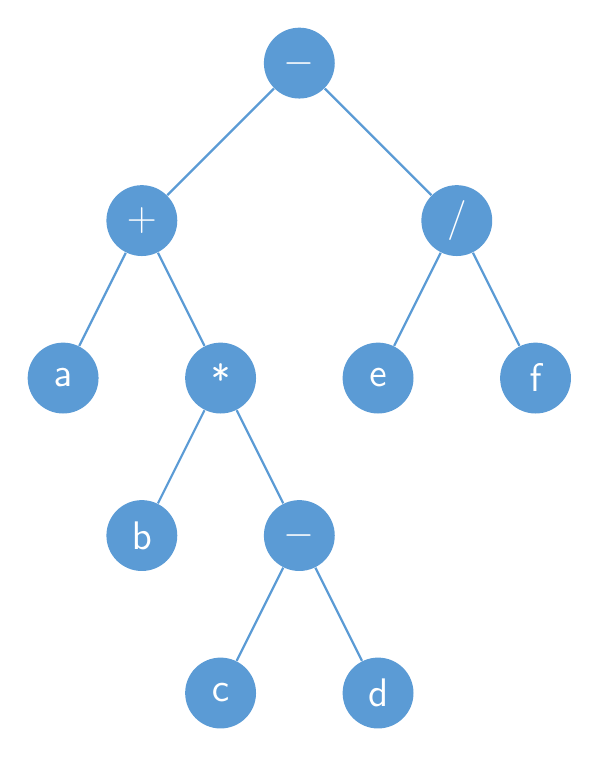
\begin{tikzpicture}[
  x=1cm,y=1cm,
  vertex/.style={circle,fill=treeblue,text=white,inner sep=0pt,
    minimum size=9mm,font=\Large\sffamily},
  edge/.style={draw=treeblue,line width=.8pt}
]
  % Expression: (a + b * (c - d)) - e / f.
  % Left and right children preserve the operand order.
  \node[vertex] (root) at (3,0) {$-$};
  \node[vertex] (sum) at (1,-2) {$+$};
  \node[vertex] (quotient) at (5,-2) {/};
  \node[vertex] (a) at (0,-4) {a};
  \node[vertex] (product) at (2,-4) {*};
  \node[vertex] (e) at (4,-4) {e};
  \node[vertex] (f) at (6,-4) {f};
  \node[vertex] (b) at (1,-6) {b};
  \node[vertex] (difference) at (3,-6) {$-$};
  \node[vertex] (c) at (2,-8) {c};
  \node[vertex] (d) at (4,-8) {d};
  \foreach \parent/\child in {root/sum,root/quotient,sum/a,sum/product,
    quotient/e,quotient/f,product/b,product/difference,difference/c,difference/d}
    \draw[edge] (\parent) -- (\child);
\end{tikzpicture}
\end{document}
